
% Do not compile, settings document 

% ========== Classe du document ==========
\documentclass[12pt]{report}    % A4, police taille 11, report pour avoir les chapitres

% ========== Langue française pour le document ==========
\usepackage{latexsym}       % Police latex de base
\usepackage[french]{babel}  % Dictionnaire français (indentation, caractères spéciaux, tirets...)
\usepackage[utf8]{inputenc} % Encodage d'entrée pour les caractères accentués
\usepackage[T1]{fontenc}    % Affichage correct des caractères accentués notamment

% ========== Géométrie du document ==========
% Gestion des différentes marges du document pour coller avec le séparateur d'en-tête
\usepackage[left=2cm , right=2cm, bottom=2cm, top=2cm, headheight=2cm, headsep=0.5cm,heightrounded=true]{geometry}
% \raggedbottom % This makes the last line of each page be at exactly the same place on the sheet of paper
% \flushbottom  % All pages will not necessarily have exactly the same height, but ‘almost the same height’
\setlength{\parskip}{1em}   % Définition de l'espace entre les paragraphes
\setlength{\parindent}{4em} % Définition de la longueur du "tab" = indentation
\usepackage{fancyhdr}       % Permet en-tête et pied de page
\pagestyle{fancyplain}      % Pour avoir le même style sur les pages fancy et sur celles plains comme la toc
\renewcommand\plainheadrulewidth{.4pt}  % Le trait noir sous les logos sur les pages plain
\fancyhead[L]{\includegraphics[scale=0.1]{Images/Grenoble-Phelma-Logo.png}}    % Logo gauche
\fancyhead[R]{\includegraphics[scale=0.03]{Images/logo-soict-hust.png}}   % Logo droit
% Redéfinir le style "empty" utilisé par le documentclass "report" pour le titre, résumé et chapitres
\fancypagestyle{empty}
{
    \fancyhf{}
    \fancyhead[L]{\includegraphics[scale=0.1]{Images/Grenoble-Phelma-Logo.png}}    % Logo gauche
    \fancyhead[R]{\includegraphics[scale=0.03]{Images/logo-soict-hust.png}} % Logo droit
}


\usepackage{afterpage} % génère ds pages blanches
\newcommand\myemptypage{
    \null
    \thispagestyle{empty}
    \addtocounter{page}{1}
    \newpage
    }

% ========== Liens dans le document, méta-datas et références ==========
\usepackage{xpatch}     % Permet de patcher certaines fonctionnalités de base comme la toc
\usepackage{float}      % Placement des flottants
\usepackage{hyperref}   % Liens dans le documents
\hypersetup{pdfborder=0 0 0} % Pas d'encadré sur les liens
\usepackage{caption}    % Légendes dans les environnements "figure" et "float"
\usepackage[list=true]{subcaption} % Légendes pour les "sous-figures" et "sous-float"
                                   % et affichage des "sous-..." dans la liste des figures
% \def\thechapter{\Alph{chapter}}    % Définition des chapitres avec une lettre
\setcounter{tocdepth}{3}           % Profondeur de numérotation de la toc  (chap > sec > subsec > subsubsec)
\setcounter{secnumdepth}{3}        % Profondeur de numérotation des titres (chap > sec > subsec > subsubsec)
\usepackage{chngcntr}              % Permet de changer les numérotations d'objets
\usepackage[titles]{tocloft}       % Gestion très précise des différentes listes

\hypersetup % Attribution des méta-datas pdf pour reconnaissance automatique Zotero entre autres
{
pdftitle={Titre},
pdfsubject={Sujet},
pdfauthor={Auteur},
pdfkeywords={keyword1} {keyword2} {keyword3}
}

% ========== Graphique, police, maths ==========
\usepackage[table,xcdraw]{xcolor}       % Package permettant d'utiliser de la couleur
% \usepackage{color}                      % Rajouter de la couleur au texte
\usepackage{bm}                         % Mettre en gras des maths avec la commande \bm
\usepackage{ragged2e}                   % Meilleure gestion de l'alignement des textes entre autres
\usepackage{tcolorbox}                  % Boite colorées pour texte, images ou équations
\usepackage{textcomp}                   % Symboles et polices
\usepackage{gensymb}                    % Symbole pour le degré entre autre
\usepackage{amsmath,amsfonts,amssymb}   % Écrire des maths
\usepackage{cancel}                     % Barrer des maths
\usepackage{mathtools}                  % Gestion des matrices et de maths complexes
\usepackage{morewrites}                 % Résoud un problème entre les listes équation et codes


\usepackage{lmodern}
\usepackage[Lenny]{fncychap}



\ChNameUpperCase
\ChNumVar{\fontsize{40}{42}\usefont{OT1}{ptm}{m}{n}\selectfont}
\ChTitleVar{\Huge \bfseries}

\usepackage{pifont}
\usepackage{enumitem}       % Gestion des énumérations

\definecolor{bulletcolor}{RGB}{0,0,0}

% \setenumerate{label=\Alph*.}
\setenumerate{label=\arabic*.}
%\setenumerate{label=\roman*.}

\setitemize{label=\textbullet, font=\Large \color{bulletcolor}}


\usepackage{siunitx}                                    % Pour des unités bien écrites
\newcommand{\nomunit}[1]{%
\renewcommand{\nomentryend}{\hspace*{\fill}#1}}         % Commande pour la nomenclature (unités à droite)
\sisetup{inter-unit-product =\ensuremath{{}\cdot{}}}    % Séparation par un point des unités
\DeclareSIUnit\bar{bar}                                 % Besoin de déclarer les bar car pas pris en charge
\DeclareSIPower\quartic\tothefourth{4}

\usepackage{contour}
\usepackage[normalem]{ulem}

\renewcommand{\ULdepth}{1.8pt}
\contourlength{0.8pt}

\newcommand{\myuline}[1]{%
	\uline{\phantom{#1}}%
	\llap{\contour{white}{#1}}%
}

% myuline on each word to allow linebreaks
\RequirePackage{xparse}
\ExplSyntaxOn
\NewDocumentCommand{\myulineX}{m}
{
	\seq_set_split:Nnn \l_tmpa_seq { ~ } { #1 }
	\seq_map_inline:Nn \l_tmpa_seq { \myuline{##1} ~ } \unskip
}
\ExplSyntaxOff

% =========== Glossaire ============
\usepackage[acronym,toc,nonumberlist]{glossaries}% pas de numéro de page dans le glossaire


\newacronym{hust}{HUST}{Hanoi University of Science and Technology : Université d'accueil}
\newacronym{bkcs}{BKCS}{Bach Khoa Cyber Security Center : Laboratoire de cybersécurité de l'université que j'ai intégré}
\newacronym{bdd}{BDD}{Base de données}
\newacronym{onvif}{ONVIF}{Open Network Video Interface Forum : Standard de communication permettant l'interopérabilité entre appareils IP}
\newacronym{ia}{IA}{Intelligence Artificielle}                        % Récupère les informations du fichier glossary.tex
\makeglossaries                         % Génère le glossaire avec les informations récupérées

% ======= Diagramme de Gantt =======
\usepackage{pgfgantt}
\definecolor{color_Gantt}{RGB}{228, 5, 32}

% ===== Gestion des figures =========
\usepackage{graphicx}               % Plus d'arguments pour la fonction \includegraphics
\graphicspath{{Images/}}            % Path des images

\counterwithin{figure}{section}     % Numérotation des figures à partir des sections
\setcounter{lofdepth}{2}            % Afficher jusqu'aux sous-figures dans la liste des figures
\cftsetindents{figure}{0em}{3.5em}  % Réglage de l'espace entre le numéro et le nom de la figure dans la liste
\setlength\cftbeforefigskip{5pt}    % Réglage de l'espacement entre les figures dans la liste
\AtBeginDocument{\renewcommand{\listfigurename}{Liste des figures}} % Renommer la liste des figures
% Ajout de la position de la liste des figures dans la toc
\xpretocmd{\listoffigures}{\addcontentsline{toc}{chapter}{\listfigurename}}{}{}

% ===== Gestion des tableaux=========
\usepackage{array,multirow,makecell}                        % Packages utiles pour les tableaux
\setcellgapes{1pt}              \usepackage{booktabs}                         % Paramètres sympa d'après Xm1Math
\makegapedcells                                             % Paramètres sympa d'après Xm1Math
\newcolumntype{R}[1]{>{\raggedleft\arraybackslash }b{#1}}   % Paramètres sympa d'après Xm1Math
\newcolumntype{L}[1]{>{\raggedright\arraybackslash }b{#1}}  % Paramètres sympa d'après Xm1Math
\newcolumntype{C}[1]{>{\centering\arraybackslash }b{#1}}    % Paramètres sympa d'après Xm1Math

\counterwithin{table}{section}      % Numérotation des tableaux à partir des sections
\setcounter{lotdepth}{2}            % Afficher jusqu'aux sous-tableaux dans la liste des tableaux
\cftsetindents{table}{0em}{3.5em}   % Réglage de l'espace entre le numéro et le nom du tableau dans la liste
\setlength\cftbeforetabskip{5pt}    % Réglage de l'espacement entre les figures dans la liste
% Ajout de la position de la liste des tableaux dans la toc
\xpretocmd{\listoftables}{\addcontentsline{toc}{chapter}{\listtablename}}{}{}

% =============== Index =============
\usepackage{imakeidx}   % Package pour créer l'index
\makeindex              % Génération de l'index
% Ajout de la position de l'index dans la toc
\xpretocmd{\printindex}{\addcontentsline{toc}{chapter}{\indexname}}{}{}

% ========== Bibliographie ==========
% Importer un fichier biblatex, sans dépassement des marges, trié par ordre d'apparition
\usepackage[block=ragged,sorting=none]{biblatex}
\usepackage{csquotes}           % Gestion des caractères " " lors des citations
\addbibresource{biblio.bib}     % Importer le fichier de bibliographie
\nocite{*}                      % Importer les éléments non cités quand même dans la bibliographie

% ===== Gestion des annexes ==========
\usepackage[toc,page,title,titletoc,header]{appendix}   % Packages indexes importants
\usepackage{pdfpages}                                   % Intégration de pdf dans le document
\renewcommand{\appendixtocname}{Annexes}      % Nom de la table des annexes dans la toc
\renewcommand{\appendixpagename}{Annexes}               % Nom du titre de la page des annexes
\usepackage{titletoc}	% Permet de générer une petite table des annexes

% ========== Utilitaires =============
\usepackage[all,defaultlines=3]{nowidow}    % Macro pour la gestion des lignes seules en bout de page
\usepackage{blindtext}                      % Génération de texte aléatoire pour les exemples

% =================== Fin Préambule Latex ====================


\begin{document}
\renewcommand{\tablename}{Tab.}
\renewcommand{\figurename}{Fig.}

% ===========    Page de Garde  ===========
% ============== Début Page de Garde ====================

\hypersetup{pageanchor=false}
\begin{titlepage}
    \begin{center}
        \vspace*{1cm}
        \Large
        Rapport de stage : Projet de Fin d’Études


        \vspace{0.5cm}
        \Huge
        \textbf{Implémentation d'un site internet de management de caméras CCTV}\\
        
        \vspace{0.5cm}
        \large
        du 01/04/2025 au 31/08/2025

        \vspace{1.5cm}
        \Large
        \textbf{BORIOS Samuel}\\
        
        \vspace{0.5cm}
        \large
        \textbf{3\ieme année PHELMA  Systèmes Embarqués Objets Connectés}\\
        \vspace{2cm}
        \textbf{Maître de stage}: Tong Van Van, vantv@soict.hust.edu.vn\\
        \textbf{Tuteur Phelma}: Nicolas Castagné, nicolas.castagne@grenoble-inp.fr\\
        
        \vspace{2cm}
        \Large
        \textbf{Rapport confidentiel}

        \vfill

\begin{figure}[H]
        \begin{subfigure}[t]{0.4\textwidth}
        \includegraphics[width=1\textwidth]{Images/Grenoble-Phelma-Logo.png}
        \centering
        \large
        3 parvis Louis Néel      38016 Grenoble
        \label{logo-Phelma}
    \end{subfigure}%
    \hfill
    \begin{subfigure}[t]{0.4\textwidth}
        \includegraphics[width=1\textwidth]{Images/logo-soict-hust.png}
        \centering
        \large
        SOICT - HUST\\
        B1 Bách Khoa, District de Hai Ba Trung, Hanoï, Vietnam
        \label{logo-entreprise}
    \end{subfigure}
    \label{logos}
\end{figure}
        \vfill
    \end{center}
\end{titlepage}

% ============ Fin Page de Garde ==================



% ===== Dos page de garde = page blanche ==
\newpage
\myemptypage

% ====== Début Préambule du rapport ========

\newpage
\hypersetup{pageanchor=true}
\setcounter{page}{1}
\tableofcontents
\listoffigures
\printglossaries



% ====== Fin du Préambule du rapport  ======



% ========== Début Document ================

\newpage

% ========== Introduction =================

\newpage
\chapter*{Introduction}
\addcontentsline{toc}{chapter}{Introduction}

Ce rapport présente le travail effectué lors de mon stage au sein du Bach Khoa Cyber Security Center (\acrshort{bkcs}) de l’Université des Sciences et Technologies de Hanoï – Hanoi University of Science and Technology (\acrshort{hust}). 
Ce stage s'inscrit dans le contexte d'un projet antérieur au laboratoire déjà complété et n'a pas pour objectif un déploiement opérationnel. Il vise principalement à expérimenter et approfondir des approches techniques liées à la surveillance vidéo et à la gestion de caméras.
Dans ce cadre, un prototype de site web a été conçu afin d’explorer des solutions de gestion et de supervision de caméras IP. Sa réalisation a constitué un support d’apprentissage, permettant d’aborder des problématiques variées telles que le développement web, le traitement de flux vidéo en temps réel et l’utilisation de protocoles de communication spécifiques à la vidéosurveillance.
Parallèlement, le stage a également permis d’approfondir des notions en cybersécurité, en qualité logicielle ainsi qu’en intelligence artificielle (\acrshort{ia}) appliquée à la détection. Ce rapport retrace les principales étapes du projet, depuis l’analyse des besoins jusqu’à la mise en œuvre d’un prototype fonctionnel, en incluant les solutions envisagées ainsi que les difficultés rencontrées.





% ========== Chapitre 1 =================
\newpage
\chapter{Contexte et objectifs du stage}


\section{Présentation du laboratoire} 

\acrshort{hust} est un acteur majeur de l’enseignement supérieur technique au Vietnam, elle a fait de la cybersécurité une priorité avec la création en 2015 du Centre de Sécurité de l’Information - \acrshort{bkcs}.

Ce centre mène des travaux de recherche appliquée dans des domaines tels que :
\begin{itemize}
	\item l’analyse de vulnérabilités systèmes,
	\item la détection d’intrusions,
	\item l’évaluation de la sécurité des infrastructures numériques.
\end{itemize}
\vspace{10px}

Il s’implique également dans le transfert technologique vers l’industrie, le soutien aux institutions publiques, la coopération internationale en recherche, et la formation des étudiants, en particulier aux niveaux master et doctorat. 

Son fonctionnement repose sur un modèle de laboratoire ouvert, réunissant des experts issus des différents instituts de recherche de l’université.





\section{Situation de départ}

Le laboratoire \acrshort{hust} - \acrshort{bkcs} est constitué de deux grands open space dont la sécurité est assurée par une simple porte fermée à clés. Ces pièces ne sont pas équipées de caméras de surveillance, ce qui pose de sérieuses questions de sécurité. 

Il m'a donc été confié le projet de recherche et de développement d'un site web qui regrouperait la vue en direct de plusieurs caméras de surveillance, ainsi que la gestion de leurs paramètres respectifs.


\section{Analyse du sujet}

Afin de préciser la direction de mes recherches j'ai d'abord étudié les solutions classiques utilisées pour une gestion de caméras de surveillance. Les principaux logiciels utilisés sont des logiciels propriétaires qui permettent de nombreuses fonctionnalités mais présentent tout de même des contre-parties : ils sont souvent chers (licences ou activations), leur déploiement peut être long et fastidieux, leur fonctionnement est fermé et ne peut être adapté.

L’objectif de mon stage était donc de rechercher les solutions pour développer un site web intuitif de gestion de caméras IP, qui permet de :

\begin{itemize}
	\item découvrir automatiquement les caméras présentes sur un réseau local,
	\item accéder facilement aux flux vidéos en direct de chaque caméra,
	\item modifier certains paramètres de configuration des caméras,
        \item le tout avec une gestion des droits utilisateurs.
\end{itemize}
\vspace{10px}

Ce travail s'inscrit dans la démarche du laboratoire de créer un outil sécurisant pour un usage interne et offrant un contrôle total sur son fonctionnement et ses données.

\section{Organisation du travail}

Mon travail n'a pas été planifié précisément au préalable mais a plutôt suivi une évolution naturelle au fil de temps et de mes recherches. Mon maître de stage m'indiquait les fonctionnalités de l'application sur lesquelles je devais me concentrer et je m'y attelait. Si je rencontrais un problème, ou bien une fois mon travail terminé, je faisais un compte rendu à mon maître de stage et il m'indiquait les fonctionnalités suivantes sur lesquelles je devait me concentrer. 

Ainsi, j'ai petit à petit fait le tour des fonctionnalités du site et ai rendu un outil fonctionnel dont mes responsables étaient satisfaits. 

\begin{table}[H]
\centering
    
%
% This reproduces an example from Wikipedia:
% http://en.wikipedia.org/wiki/Gantt_chart
%
\definecolor{barblue}{RGB}{153,204,254}
\definecolor{groupblue}{RGB}{51,102,254}
\definecolor{linkred}{RGB}{165,0,33}
\renewcommand\sfdefault{phv}
\renewcommand\mddefault{mc}
\renewcommand\bfdefault{bc}
% \setganttlinklabel{s-s}{START-TO-START} % à activer si vous souhaiter faire des liens entre les tâches
% \setganttlinklabel{f-s}{FINISH-TO-START}
% \setganttlinklabel{f-f}{FINISH-TO-FINISH}
\sffamily
\begin{ganttchart}[
    canvas/.append style={fill=none, draw=black!5, line width=.75pt},
    hgrid style/.style={draw=black!5, line width=.75pt},
    vgrid={*1{draw=black!5, line width=.75pt}},
    % today=20,
    today rule/.style={
      draw=black!64,
      dash pattern=on 3.5pt off 4.5pt,
      line width=1.5pt
    },
    today label font=\small\bfseries,
    title/.style={draw=none, fill=none},
    title label font=\bfseries\footnotesize,
    title label node/.append style={below=7pt},
    include title in canvas=false,
    bar label font=\mdseries\small\color{black!70},
    bar label node/.append style={left=0.5 cm},
    bar/.append style={draw=none, fill=blue!63},
    bar incomplete/.append style={fill=barblue},
    bar progress label font=\mdseries\footnotesize\color{black!70},
    group incomplete/.append style={fill=groupblue},
    group left shift=0,
    group right shift=0,
    group height=.5,
    group peaks tip position=0,
    group label node/.append style={left=.6cm},
    group progress label font=\bfseries\small,
    link/.style={-latex, line width=1.5pt, linkred},
    link label font=\scriptsize\bfseries,
    link label node/.append style={below left=-2pt and 0pt}
  ]{1}{22}
  \gantttitle[
    title label node/.append style={below left=7pt and -3pt}
  ]{Semaines:\quad1}{1}
  \gantttitlelist{2,...,22}{1} \\
  \ganttgroup{Recherche et réalisation}{1}{12} \\
  \ganttbar{\textbf{T 1.1} Développement web}{1}{3} \\
  \ganttbar{\textbf{T 1.2} Gestion utilisateurs}{2}{4} \\
  \ganttbar{\textbf{T 1.3} Flux vidéos et intégration}{4}{9} \\
  \ganttbar{\textbf{T 1.4} Gestion paramètres internes}{10}{12}
  \\[grid]
  
  \ganttgroup{Travaux supplémentaires}{13}{17} \\
  \ganttbar{\textbf{T 2.1} Analyse qualité code}{13}{14} \\
  \ganttbar{\textbf{T 2.2} IA de détection}{15}{17} \\
    
  \ganttgroup{Archivage, rapports}{18}{22}\\
  \ganttbar{\textbf{3.1} Rédaction rapport de stage}{18}{20}\\
  \ganttbar{\textbf{3.2} Préparation soutenance}{21}{22}
  
%   \ganttlink[link type=s-s]{WBS1A}{WBS1B}
%   \ganttlink[link type=f-s]{WBS1B}{WBS1C}
%   \ganttlink[
%     link type=f-f,
%     link label node/.append style=left
%   ]{WBS1C}{WBS1D}
\end{ganttchart}



\caption{Diagramme de Gantt réalisé}
\label{tab:diag de Gantt}
\end{table}


% ========== Chapitre 2 =================
\newpage
\chapter{Recherches et réalisations}

\section{Développement d'un site web}

Mon maître de stage m'a dit que je pouvais développer le site dans le langage que je voulais. Je n'ai cependant jamais développé de site web, j'ai donc cherché comment faire pour commencer.

Je me suis d'abord intéressé aux langages de programmation de sites web comme HTML, CSS ou JavaScript. J'ai fait quelques tutoriels pour essayer de me familiariser avec ces derniers mais cela n'allait pas très loin sans des outils externes.

Je me suis donc intéressé aux frameworks, afin de me permettre de me concentrer rapidement sur le développement des fonctionnalités de mon site sans avoir besoin de créer l'infrastructure de base du site. Il en existe un très grand nombre : ceux utilisés dans l'industrie (comme React, Angular, etc..) qui sont assez complexes à prendre en main, ceux dit "full-stack" (comme Next.js) qui sont très complet mais peuvent aussi être déconseillés aux débutants, et enfin les frameworks générateurs de sites statiques qui sont simples, rapides et moins adaptés aux applications complexes. 

J'ai choisi l'un de ces derniers pour développer mon site : Astro \cite{astro}, car je n'avais pas besoin de m'embêter avec des frameworks complexes inutilement. Astro permet de créer des interfaces propres avec peu de code, tout en gardant la possibilité d’intégrer des composants dynamiques si nécessaire. Ce choix m'a paru viable pour continuer mon projet et mon maître de stage ne m'a pas déconseillé de continuer alors je suis passé à la suite rapidement après avoir pris en main ce framework.

\newpage
\section{Gestion des utilisateurs}

Pour que le site soit sécurisé il est important de gérer correctement les utilisateurs qui y ont accès, ma priorité a donc été de chercher à implémenter ça pour commencer. 

J'ai donc cherché dans la documentation Astro pour savoir si une telle fonctionnalité était facilement implémentable. J'ai trouvé directement Supabase \cite{supabase}, plateforme open-source compatible avec Astro qui permet de mettre en place des bases de données (\acrshort{bdd}) PostgreSQL facilement pour des applications web sans se soucier de l'infrastructure backend. Je me disais au départ que je stockerai les login et mots de passe dans une \acrshort{bdd} Supabase pour gérer les utilisateurs du site, mais il se trouve que Supabase gère l'authentification aux bases de données directement, je n'ai donc pas eu le besoin de faire ces \acrshort{bdd}.


\section{Accéder au flux en direct de la caméra et l'intégrer sur le site}

Les caméras dont je devais m'occuper sont des caméras IP, elles émettent en continu un flux rtsp, appelé ainsi car on peut accéder à leur live via une adresse "rtsp:// adresseIP: port". Il est facile de tester une telle connexion via VLC en rentrant l'adresse complète suivant le template précédent. Le problème est l'intégration d'un tel flux en direct sur un site web, c'est là que la majorité de mon temps de recherche a été consacré. 

Le principal problème était de trouver un moyen de convertir le flux rtsp en un format compatible web \cite{webrtc}, le tout en assurant une connexion sécurisée https au lieu d'un http simple. J'ai pallié ce problème intuitivement en utilisant des certificats auto-signés, qui m'ont permis de créer une connexion pseudo sécurisée. Ce n'est évidemment pas viable pour une application professionnelle mais pour l'instant cela m'a permis de continuer mes recherches, nous y reviendrons plus tard. Les solutions que j'ai testé ensuite pour convertir mon flux rtsp sont nombreuses (Janus, Plugin VLC, IpCamLive, Kurento, etc) mais la majorité d'entre elles ne convenaient pas. Le principal souci rencontré a été la difficulté d'installation et le fait que ces solutions ne soient pas facilement automatisables ou intégrées dans une page web externe (mon site). Après donc beaucoup de recherches je me suis arrêté sur la solution suivante : un serveur RTSPtoWeb \cite{rtsptoweb}. Ce serveur est open source, facilement installable et modifiable, s'intègre simplement sur d'autre sites et surtout s'automatise parfaitement, il permet donc une très bonne scalabilté avec plus de caméras. Il me suffit de le lancer sur Docker avec une simple commande et il peut tourner en arrière plan son mon propre ordinateur et fournir la passerelle nécessaire entre mes caméras et mon site web.

J'ai donc maintenant accès au flux en direct de mes caméras sur mon site sans délai et avec une très bonne qualité, les dernières fonctionnalités qu'il me reste à implémenter sont les modifications de certains paramètres des caméras.

\section{Gestion des paramètres internes des caméras}

Pour cette partie mon maître de stage m'a conseillé d'utiliser le standard Open Network Video Interface Forum (\acrshort{onvif}) \cite{onvif}. C'est un standard de communication qui assure l'interopérabilité entre dispositif de vidéosurveillance IP. Je vais l'utiliser ici pour deux fonctions principales : la détection automatique de caméras sur le réseau et la configuration de ces dernières.

J'ai commencé par écrire plusieurs fichiers de test pour toutes les fonctions \acrshort{onvif} que j'avais rencontré et qui me semblaient utiles. En effet en fonctions des caméras et de leur configurations, certaines fonctionnalités \acrshort{onvif} sont parfois accessibles ou non. La conclusion de tout ces tests est donc la suivante : j'ai bien la possibilité de modifier les paramètres d'encodage vidéo et les paramètres de gestion utilisateurs mais je n'ai accès à aucune des fonctionnalités liées aux enregistrements vidéo. Le fait que je n'ai pas accès aux enregistrements vidéos a posé problème car il était prévu à la base que l'on puisse accéder à ces derniers via mon site. J'ai passé plusieurs semaines à chercher une solution à ce problème avec mon maître de stage mais nous nous sommes mis d'accord pour abandonner cette idée car elle était trop demandante selon lui.

Tout de même très satisfait des paramètres vidéo et utilisateurs j'ai développé une page des paramètres très complète sur mon site, j'ai également pu faire la page d'accueil qui détecte les caméras présentes sur le réseau sans problème. 


% ========== Chapitre 3 =================
\newpage
\chapter{Travaux supplémentaires}

\section{Analyse de qualité du code}

Une fois mon travail terminé, le site fonctionnel et les rapports rendus (manuel utilisateur, diagrammes fonctionnels, etc) mon responsable m'a conseillé de lancer mon projet sur une machine virtuelle et d'y effectuer des tests via SonarQube \cite{sonarqube} pour tester la qualité de mon code. SonarQube est une plateforme open source d'analyse de qualité de code, elle permet aux développeurs d'améliorer la qualité, la maintenabilité et la sécurité de leurs applications. En effet j'ai, grâce aux analyses de SonarQube, corrigé de nombreux problèmes dans mon code, allant des bugs aux variables inutilisées, en passant par les duplications de code. 

\section{Usage de l'intelligence artificielle}

Après avoir confirmé avec mon maître de stage que tout était correct il m'a proposé de continuer sur ma lancée et de faire des recherches sur les \acrshort{ia} de détection ainsi que leur utilisation dans la télésurveillance. Mon objectif premier était de trouver un modèle d'\acrshort{ia} qui me permettrait de détecter et de compter les personnes présentes dans le bureau pour un enregistrement donné. 

La première étape était de faire en sorte de corriger l'effet "fisheye" de la caméra afin d'avoir une image ou la perspective n'est pas modifiée pour que l'\acrshort{ia} puisse travailler dans de bonnes conditions. Pour ce faire j'ai écrit un programme qui corrige la déformation de chaque image de mon enregistrement vidéo, j'ai trouvé les paramètres de déformations corrects de manière empirique.

Une fois cela fait, j'ai pu commencé à télécharger des modèles d'\acrshort{ia} pré-entraînés à détecter des gens et à les tester sur mon enregistrement. Après plusieurs tests et itérations je suis arrivé à un résultat très concluant en utilisant le modèle CrowdHuman YOLOv5m \cite{yolo,shao2018crowdhuman}. Il repose sur l’architecture YOLOv5m, une variante de taille moyenne de YOLO (algorithme de détection d’objets en temps réel) qui équilibre vitesse et précision. Ce modèle CrowdHuman est donc un modèle YOLOv5 qui a été entraîné au préalable sur un dataset complet de foules et de scènes où les gens ne sont pas facilement reconnaissables. C'est particulièrement pertinent ici car les modèles de reconnaissance non entraînés avaient du mal à reconnaître mes collèges derrière leurs écrans d'ordinateur et tout les élément occluant que l'on peut retrouver dans un openspace. 

Le résultat final que j'ai obtenu est très concluant et assez rapide à compiler, cf Fig. \ref{fig:crowdhuman}. On voit bien que le modèle reconnaît la majorité des personnes présentes sur l'image et peut situer leur tête correctement. Il y a plein d'objets obstruant la vue de la caméra mais la détection se fait sans souci, les seules personnes que le modèle ne reconnaît pas sont très loin de la caméra et à peine reconnaissables à l’œil nu.

\begin{figure}[H]
    \centering
    \includegraphics[width=0.7\textwidth]{Images/yolov5crowdhuman.png}
    \caption{Reconnaissance de personnes via CrowdHuman}
    \label{fig:crowdhuman}
\end{figure}



% ========== Conclusion =================
\newpage
\addcontentsline{toc}{chapter}{Conclusion et perspectives}
\chapter*{Conclusion et perspectives}

Ainsi ce stage m’a permis de mettre en pratique mes connaissances tout en découvrant de nouveaux outils et méthodes liés au développement web et à la télésurveillance. J’ai conçu un site fonctionnel de gestion de caméras IP intégrant l’authentification des utilisateurs, l’accès en direct aux flux vidéos et la configuration des paramètres via le standard \acrshort{onvif}. Ce projet a atteint ses objectifs et constitue une base solide pour de futurs développements, il y a toutefois certaines limitations techniques à ne pas ignorer. 

En effet, le serveur utilisé pour la gestion de mes flux vidéos (RTSPtoWeb) est un serveur open source qui fonctionne parfaitement pour notre utilisation, mais il a aussi ses limites : : le service n’intègre ni authentification ni gestion native des accès, il repose sur la solidité de ma configuration Docker et expose des ports sensibles qui, mal protégés, pourraient ouvrir la porte à des intrusions. Ce choix de serveur donne un contrôle total sur les données, mais à condition de le renforcer, voici quelques perspectives d'améliorations : un reverse proxy, un chiffrement HTTPS valide, une authentification, et idéalement un VPN ou un filtrage d’IP. Sans ces mesures, le déploiement actuel reste insuffisant pour sécuriser des flux CCTV sensibles.





% ========== Bibliographie =====================

\newpage
\printbibliography[heading=bibintoc]

% =========Fin Biblio ==========================

% ========= Début Annexes ======================

\begin{appendices}

\chapter{Résumé en français}

Lors de mon stage au \acrshort{bkcs} - \acrshort{hust}, j’ai eu pour mission de concevoir et développer un site web de gestion de caméras IP afin de renforcer la sécurité du laboratoire. L’application devait permettre la découverte automatique des caméras sur le réseau local, l’accès aux flux vidéo en direct, la modification de certains paramètres et une gestion sécurisée des utilisateurs.

Pour répondre à ces objectifs, j’ai choisi le framework Astro pour le développement web, associé à Supabase pour l’authentification et la gestion des utilisateurs. J’ai intégré le serveur RTSPtoWeb afin de diffuser les flux vidéo en direct et utilisé le standard \acrshort{onvif} pour la détection et la configuration des caméras. Bien que la fonctionnalité d’accès aux enregistrements vidéo n’ait pas pu être implémentée, le site final a rempli les attentes principales de mes responsables.

En complément, j’ai réalisé une analyse de la qualité du code avec SonarQube et mené des recherches sur l’utilisation de l’intelligence artificielle dans la vidéosurveillance. L’intégration du modèle CrowdHuman YOLOv5m m’a permis d’obtenir des résultats fiables pour la détection et le comptage de personnes en temps réel dans un environnement de type open space.

Ce stage m’a permis de renforcer mes compétences en développement web, cybersécurité et intelligence artificielle tout en contribuant à un projet concret et utile. Il a constitué une expérience formatrice, tant sur le plan technique que professionnel.

\chapter{English summary}

During my internship at \acrshort{bkcs} - \acrshort{hust}, I was assigned to design and implement a web-based system for managing IP cameras in order to improve the laboratory’s security. The project involved developing an intuitive website capable of discovering cameras on a local network, providing live video streams, and allowing the configuration of various camera parameters while ensuring secure user authentication.

To achieve this, I first explored web development frameworks and chose Astro for its simplicity and flexibility. I integrated Supabase for user management, deployed RTSPtoWeb to handle live video streaming, and used the ONVIF standard for camera detection and configuration. Although video recording management could not be implemented due to technical limitations, the final tool successfully delivered the essential functionalities expected by my supervisors.

Beyond the core development, I performed code quality analysis with SonarQube to enhance maintainability and security, and I conducted research on artificial intelligence applied to video surveillance. By testing and adapting the CrowdHuman YOLOv5m model, I achieved reliable real-time people detection within office environments.

This internship allowed me to strengthen my technical skills in web development, cybersecurity, and AI applications while contributing to a concrete solution for the laboratory’s security needs.


\chapter{Rendus transmis à mon responsable à la fin de mon travail}

\section{Manuel utilisateur du site}

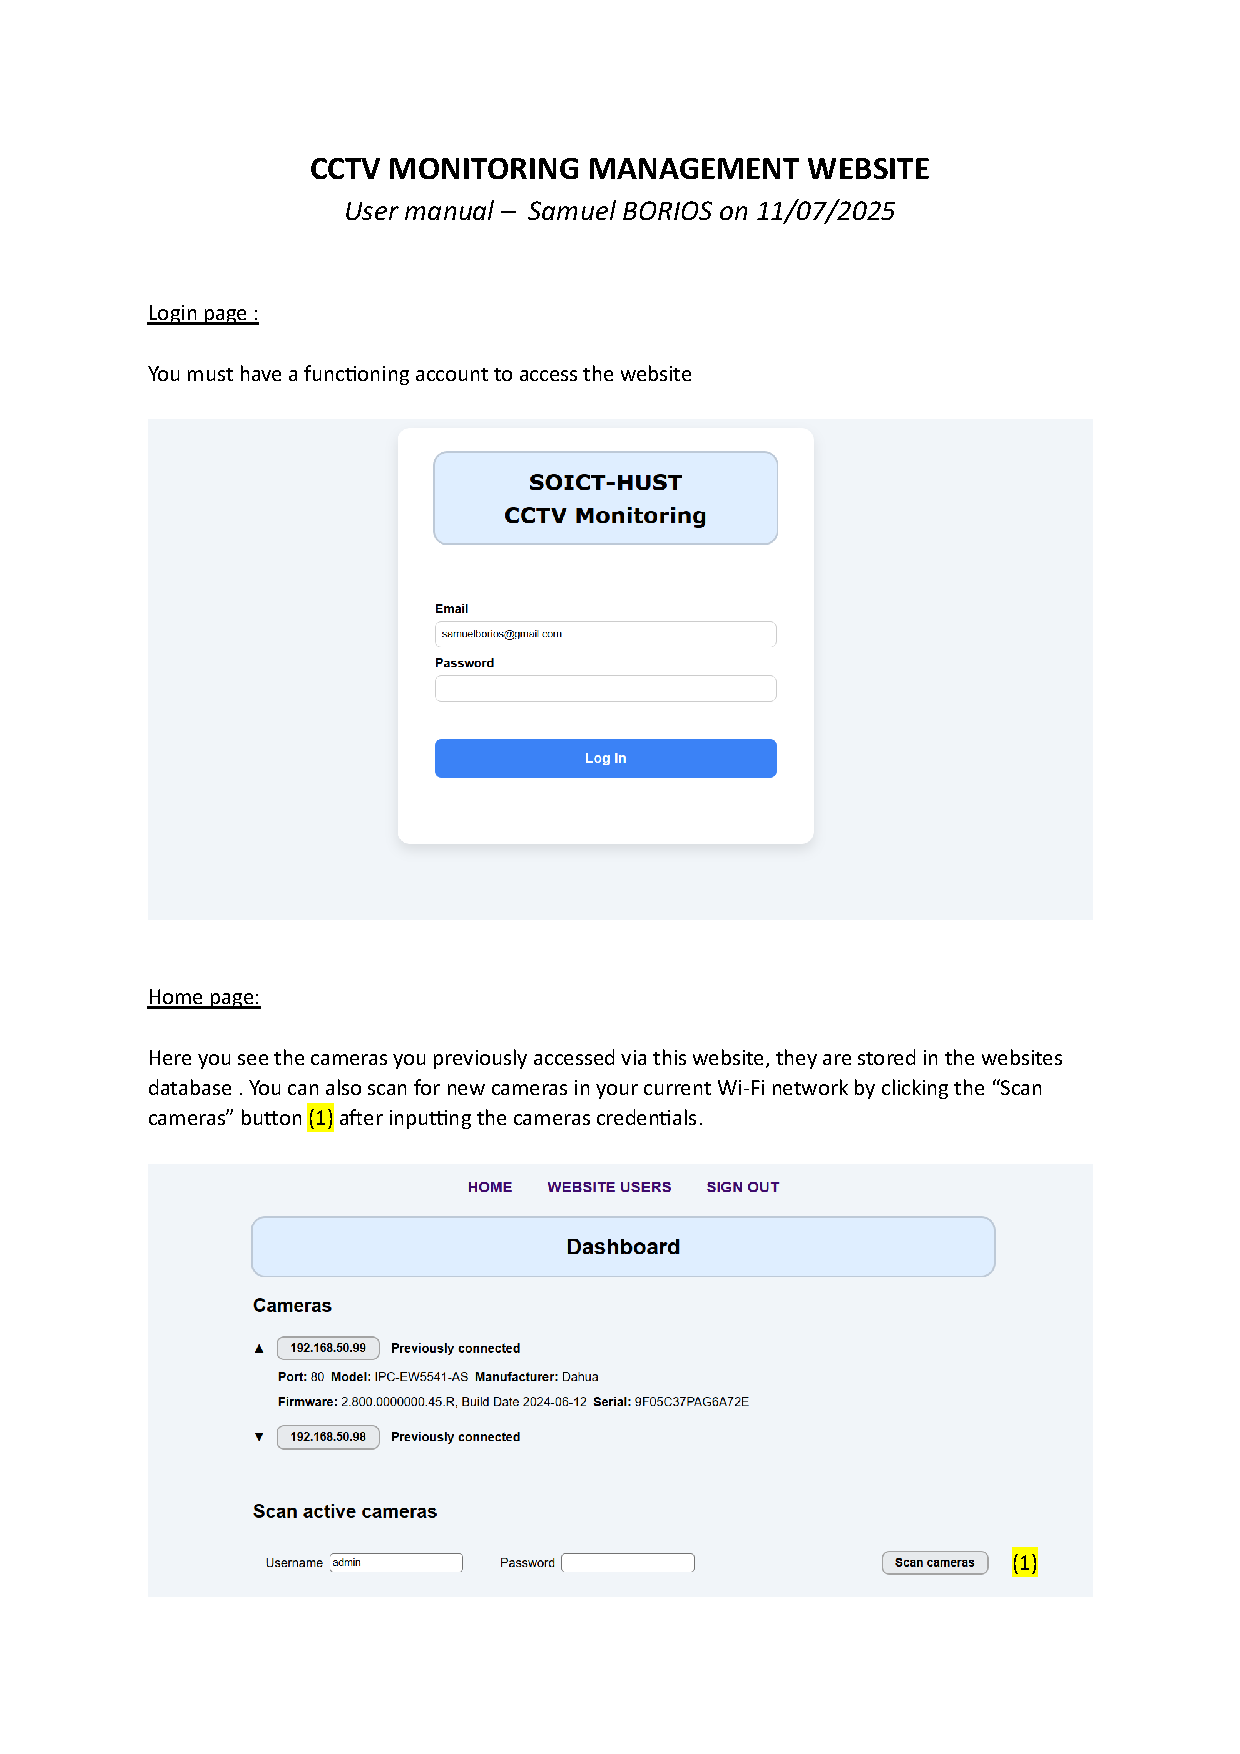
\includepdf[pages=1, trim=0cm 2cm 0cm 6cm, clip]{User manual - CCTV Website.pdf}
\includepdf[pages=2-]{User manual - CCTV Website.pdf}

\section{Diagrammes d'architecture système}

\begin{figure}[H]
    \centering
    \includegraphics[width=0.55\textwidth]{Images/Functionnal diagram.png}
    \caption{Diagramme fonctionnel}
    \label{fig:functdiag}
\end{figure}

\begin{figure}[H]
    \centering
    \includegraphics[width=0.55\textwidth]{Images/System deployment diagram.png}
    \caption{Diagramme de déploiement}
    \label{fig:systdepldiag}
\end{figure}


\chapter{Fiche-archive de stage}

% ============== Début Page de Garde ====================

\hypersetup{pageanchor=false}
\begin{titlepage}
    \begin{center}
        \vspace*{1cm}
        \Large
        Rapport de stage : Projet de Fin d’Études


        \vspace{0.5cm}
        \Huge
        \textbf{Implémentation d'un site internet de management de caméras CCTV}\\
        
        \vspace{0.5cm}
        \large
        du 01/04/2025 au 31/08/2025

        \vspace{1.5cm}
        \Large
        \textbf{BORIOS Samuel}\\
        
        \vspace{0.5cm}
        \large
        \textbf{3\ieme année PHELMA  Systèmes Embarqués Objets Connectés}\\
        \vspace{2cm}
        \textbf{Maître de stage}: Tong Van Van, vantv@soict.hust.edu.vn\\
        \textbf{Tuteur Phelma}: Nicolas Castagné, nicolas.castagne@grenoble-inp.fr\\
        
        \vspace{2cm}
        \Large
        \textbf{Rapport confidentiel}

        \vfill

\begin{figure}[H]
        \begin{subfigure}[t]{0.4\textwidth}
        \includegraphics[width=1\textwidth]{Images/Grenoble-Phelma-Logo.png}
        \centering
        \large
        3 parvis Louis Néel      38016 Grenoble
        \label{logo-Phelma}
    \end{subfigure}%
    \hfill
    \begin{subfigure}[t]{0.4\textwidth}
        \includegraphics[width=1\textwidth]{Images/logo-soict-hust.png}
        \centering
        \large
        SOICT - HUST\\
        B1 Bách Khoa, District de Hai Ba Trung, Hanoï, Vietnam
        \label{logo-entreprise}
    \end{subfigure}
    \label{logos}
\end{figure}
        \vfill
    \end{center}
\end{titlepage}

% ============ Fin Page de Garde ==================



\section{Descriptif de stage (anglais):}

With the growing number of CCTV cameras, managing each camera manually becomes impractical. The need for a centralized management system is essential to streamline surveillance and enhance security. 

The main goal of this internship is to develop an efficient system for managing multiple CCTV cameras. Manually monitoring large numbers of cameras is not feasible, so automation is necessary. In addition to the management system, AI can be integrated to analyze video streams and detect anomalies, such as theft, fires, or other security threats. 

Here are the main functions of the website that need to be implemented :

\begin{table}[H]
\centering
\begin{tabular}{|c|l|p{8cm}|}
\hline
\# & Function & Description \\ \hline
1 & Login & Login to Web interface with account and password \\ \hline
2 & Logout & Logout of Web interface \\ \hline
3 & Scan camera in LAN network & Scan for available Camera devices in the network using ONVIF standard \\ \hline
4 & Configuration management & Collect and display information of camera device. Allows remote control of camera device, turning on/off device. \\ \hline
5 & View video stream & Allows viewing of camera video stream directly via RTP protocol \\ \hline
6 & Store video stream & Allows video storage from camera devices \\ \hline
\end{tabular}
\caption{Website functions to be implemented}
\label{tab:websitefunct}
\end{table}

\section{Moyens et encadrements mis à disposition:}

Pour ce stage le laboratoire a mis en place une caméra IP dans le bureau ainsi qu'un réseau Wi-Fi indépendant auquel j'ai pu me connecter pour accéder directement à la caméra. Cela m'a permis de travailler dans un environnement stable et contrôlé. 

De plus, j'ai rapidement pris contact avec mes collègues et mon responsable m'a conseillé de ne pas hésiter leur demander de l'aide. J'ai donc tout au long de mon stage communiqué avec M. Dong Le Van, spécialisé dans la sécurité réseau, qui a su m'aider et répondre à mes questions. J'ai également reçu des conseils de M. Cuong Dao Viet pour tout ce qui touche aux \acrshort{ia} de détection.

\end{appendices}

% ============= Fin Annexes =====================

\end{document}

